\documentclass{article}
\usepackage[margin=1.0in]{geometry} % smaller margin for document
\usepackage[margin=.7in]{caption} % little more margin for captions to make look nice
\usepackage{graphicx}
\usepackage[counterclockwise, figuresleft]{rotating} % get the heatmap rotated correctly

\title{The effect of pipeline-collection-diversity on performance}

\author{Sean Carver @ Data Machines Corporation}

\begin{document}

\maketitle

\abstract{Do performers who submit \emph{diverse} collections of
  pipelines tend to perform better than those who submit less diverse
  collections of pipelines? The answer for the Winter 2020 evaluation
  is effectively no. While there does exist a statistically
  significant effect of increased diversity on increased score, the
  effect size is trivial. Thus, it seems that less diverse collections
  of pipelines, i.e. those that focus more on hyperparameter tuning,
  can be as effective (or almost as effective, on average) as those
  that explore a greater diversity and/or ordering of primitives. }

\section{Introduction}
In section \ref{sec:measures}, \emph{Measures of Diversity}, we define
several measures of the diversity within a collection of three or more
pipelines. In section \ref{sec:glance}, \emph{Results at a Glance}, we
present a heat map showing briefly the (weak) connection between
diversity and performance. In section \ref{sec:quantifying},
\emph{Quantifying the Effect of Diversity}, we report on regression
results which point to the measurable, though substantively trivial,
effect of diversity on score. In a final section
\ref{sec:visualization}, \emph{Visualizing Collections} we show a
visualization of collections of pipelines for a problem together with
a multiple alignment, for context.

\section{Measures of Diversity}
\label{sec:measures}
Before we can define \emph{diversity} of a collection of (say 3 to 20)
pipelines, we first need to define the distance between a pair of
pipelines.  We choose the Levenshtein edit distance as this measure
between two pipelines.  Specifically, we first express the pipelines
as sequences of primitives, where primitives are written as
``letters'' in a large alphabet.  The software we use accommodates all
D3M primitives with two-letter pairs, each pair representing a single
token (primitive) of the alphabet.  The Levenshtein edit distance is
the minimum number of substitutions, insertions and/or deletions
needed to bring one sequence to coincide with the other.  This measure
satisfies the axioms for a distance.

But \emph{distance} involves just two pipelines; \emph{diversity}
measures variation among a collection of three or more pipelines.  We
tried several alternatives for quantifying diversity.  The most
well-behaved measures (i.e.\ the ones that behave most closely to our
expectations on synthetic data) were vector norms where the vector
components were the Levenshtein distances for all possible unordered
pairs of pipelines in the collection.

More precisely, we used $l_p$ norms where $p$ was a parameter varying
between 1 and $\infty$.  The different norms measure slightly different
quantities.  At the extreme, the $l_\infty$ norm (maximum
edit-distance component) is large when there is at least one pair of
pipelines at great distance, regardless of the positions (great or
small) of the other as-close or closer distances.  On the other hand,
the $l_1$ norm (sum of the edit-distance components) can still be
relatively large if there are many pairs pipelines at moderate
distance, even though there is no pair at great distance.  We point
out that the choice the different norms can sometimes matter: we have
noted that the choice can order sets of collections---synthetic or
real---differently in terms of diversity.

%Note that absolute values found in textbook definitions of the $l_p$
%norm:
%$$l_p([v_1,\dots,v_n]) = \sqrt[p]{|v_1|^p + \dots + |v_n|^p}$$ remain
%unnecessary because all distances (e.g.\ the Levenshtein edit distance
%components of $v$) must be non-negative by the properties of distance.

In the $l_p$ norm, what value for the parameter $p$ do we pick?  If
you are using only one measure of diversity, we recommend the $l_2$
norm as a nice trade off between the two extremes.  That said, it is
more informative to report two or more measures of diversity, in which
case $l_1$ and $l_\infty$ should be preferred because they are most
independent.

\section{Results at a Glance}
\label{sec:glance}
Figure \ref{fig:heatmap} shows the diversity of performer pipeline
submissions by problem type. The color-coding indicates diversity,
with purple colors indicating small $l_2$ edit distance norms,
trending towards yellow colors indicating larger $l_2$ edit distance
norms.The number of asterisks in each cell captures the count of times
a pipeline in that performer-category was the best (or tied). For
instance, in the second row of the first column, UCB twice had the
best-performing pipeline on a data set in the binary\_classification
problem category. Overall, the figure suggests (and we quantify below)
a very small but measurable effect of diversity.

% the [h] asks LaTeX to keep the image Here
\begin{sidewaysfigure}
% typically cenetered
\centering
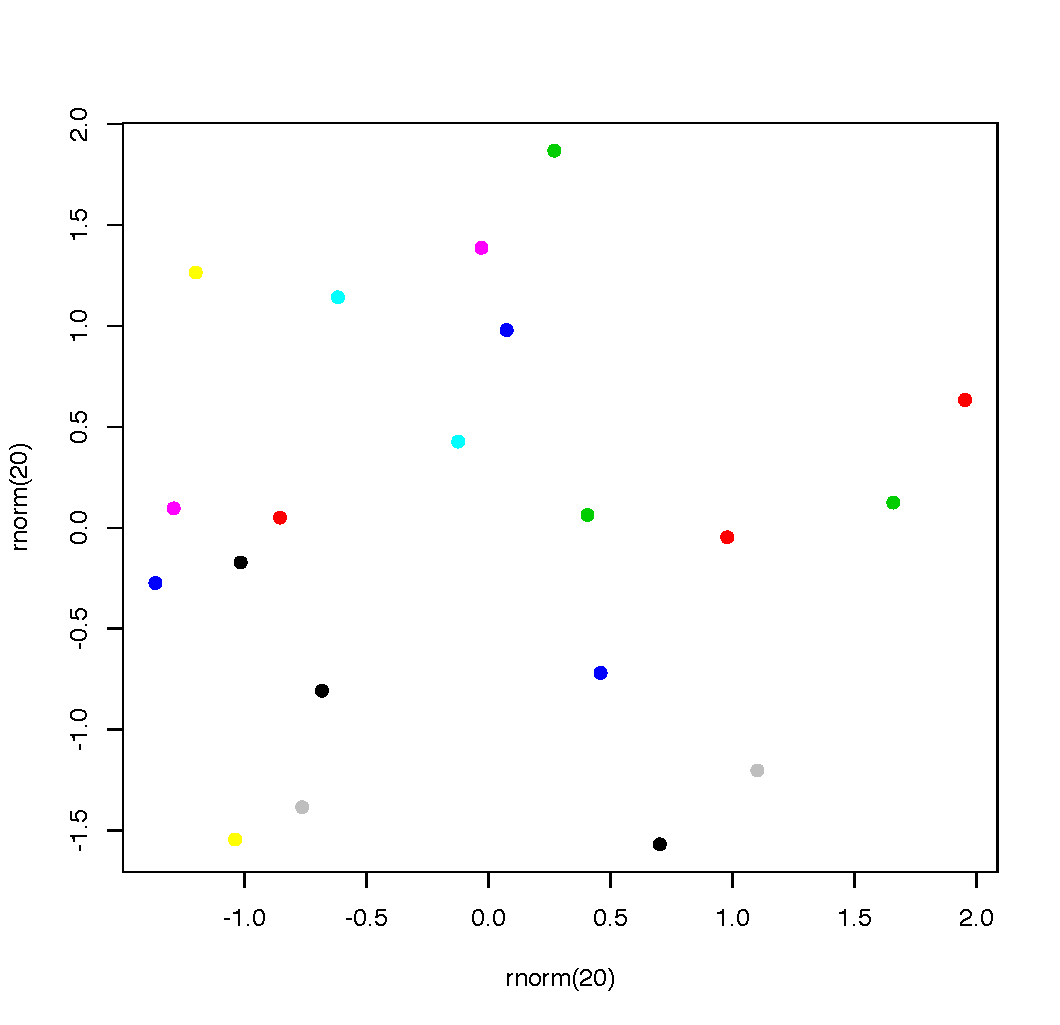
\includegraphics[scale=1.3]{heatmap.pdf}
\caption{Heat map of $l_2$ diversity see section ``Measures of
  Diversity'' for a discussion of this and other measures we use to
  quantify diversity.  The horizontal axis is the problem category and
  the vertical axis is performer for the Winter 2020 evaluation.  The
  number of asterisks in each cell is the number of problem instances
  in the corresponding category-performer which was the best (or tied
  for best) performing pipeline for any problem.  There were 37 ties
  (including multi-way ties), corresponding to an additional 37
  asterisks in the figure beyond the total number of 103 problems.}
\label{fig:heatmap}
\end{sidewaysfigure}

\section{Quantifying the Effect of Diversity}
\label{sec:quantifying}
We use regression-based methods to quantify the effect of diversity on
performance.  We address complications by combining several
overlapping methodologies.  Overall, our goal is to specify predictive
models of performance.  Our unit of analysis is a collection of
pipelines submitted by a performer for a particular problem.  The
response variable is the best score of all pipelines in the
collection.  Our models predict best score based on three explanatory
variables: the $l_1$ and $l_\infty$ norms for the collection (as
discussed above), as well as ``count,'' the number of pipelines in the
collection.

The fact that different metrics were used for scoring different
problems forced us to make adjustments.  In some cases the best score
was the greatest score, whereas in others the best score was the least
score.  By reversing the sign where appropriate, we transform scores
so that greatest score was always best score.  Our response variable
was then called ``max\_score.''

The fact that max\_scores were on widely different scales across
problems forced us to switch to standardized coordinates (z-scores)
for max\_score.  The population for this standarization was all
collections for all performers for one particular problem---as these
were guaranteed to have metrics on the same scale.

At this point, we also transformed the predictor variables to
standardized coordinates (against the same population), making
predictors comparable only to other predictors for that problem.

Below, we report on five classes (A-E) of statistical models.  For the
purposes of analysis, we grouped problems by eleven categories
(e.g.\ time series, binary classification, etc).  See the horizontal
axis of Figure 1 for a list of our categories.

In the first model, we group all problem categories together for
analysis in a ``complete pooling'' model; see MODEL A.  In the second,
we ran a fixed effects model (MODEL B) on category.  Third, we then
ran a no pooling model (MODEL C), which is actually numerous separate
models, one for each category.  We then ran a hierarchical model with
random effects on the intercept (MODEL D).  Finally, we ran a
hierarchical model with random effects on both the intercept and slope
(MODEL E).

In all models, we see that there is a significant effect of $l_1$
z-score diversity on performance, but the coefficient is small (less
than .2).  The fact that we are using z-scores for both the predictors
and response variable complicates the interpretation of this result.
What it says is that for an increase of z-score of the predictor
variable ($l_1$ z-score) by 1 the model predicts that the response
variable (max\_score z-score) will increase by almost 0.2.  Put
another way when the raw $l_1$ increases by one standard deviation for
that problem, max\_score increases by almost 0.2 standard deviations
for that problem.

It is helpful to translate this result into raw scores for $l_1$.  A
unit increase in $l_1$ means an one extra substitution, insertion, or
deletion is needed to bring just one pair of pipelines to coincidence.
We keep z-scores for max\_score because raw scores for max\_scores are
meaningless for across-problem comparison.  To convert to a
transformation from a unit increase in raw $l_1$ to a specified
z-score increase of max\_score, we must divide the coefficient (about
0.2, depending on model) by the standard deviation of $l_1$ for the
population referenced by the z-score.  Of course, each problem has a
different reference population so each problem has a different
standard deviation.  By implication, the transformed slopes will be
different for each problem, but we can obtain summaries of the
distribution of these slopes.

The 5-number summary of this distribution of slopes is
$$[0.00037622, 0.00052519, 0.00067828, 0.00114945, 0.00809511],$$
showing that a unit increase in $l_1$ leads to at most a 8-thousanths
increase in the z-score of max\_score, and the increase is usually
quite a bit less.  Our conclusion is that diversity has a negligibly
small effect on performance.

Table 1 summarizes our results.

\begin{table}
  \begin{tabular}{c|c|c|c|c}
    Model & Coefficient & p-value & estimate & std error \\
    A  & $l_1$ (z-score) & 0.00716 ** & 1.984e-01 & 7.355e-02 \\
    B  & $l_1$ (z-score) & 0.00763 ** & 1.984e-01 & 7.414e-02 \\
    C  & $l_1$ (z-score) & multiple models, same story. & & \\
    D  & $l_1$ (z-score) & 0.00716 ** & 1.984e-01 & 7.355e-02 \\
    E  & $l_1$ (z-score) & 0.0155  *  & 1.778e-01 & 7.329e-02 \\
  \end{tabular}
  \caption{Summary of models predicting the z-score of a performer's
    best score in a submitted collection, based on $l_1$ and
    $l_\infty$ measures of diversity of the collection and count of
    number of pipelines in the collection.  We performed a regression
    analysis with 5 different models (A-E, see text).  The table
    shows the model, the coefficient examined (in this case, always
    considered just $l_1$, among other predictors we used: $l_\infty$
    and count).  Furthermore, the table shows p-values (two tailed,
    under the null hypothesis that coefficient is zero), estimates of
    coefficients and standard errors of the estimates.  Note that
    several entries of the table are identical to our numerical
    precision.  We attribute this result to category-level predictors
    that do not covary with response variable.  We examine the effect
    of colinearity between $l_1$ and $l_\infty$ and found that it did
    not change our results substantially. Significance codes: 0
    ``***'' 0.001 ``**'' 0.01 ``*'' 0.05 ``.''  0.1 \emph{[blank]} 1.}
\end{table}

\section{Visualizing Collections}
\label{sec:visualization}
In this final section, we show a cartoon visualization of collections
of pipelines for a problem together with a multiple alignment (see
Figure 2, and its caption).

\begin{figure}
\centering

\includegraphics{seebelow.pdf}
\caption{The next several pages show a cartoon figure of a multiple
  sequence alignment of all submitted pipelines (all performers) for
  one randomly selected problem {\bf
    semi\_1217\_click\_prediction\_small\_MIN\_METADATA}.  The circles
  in the first pane illustrate the pipelines and are referenced with
  the number that corresponds to the label in the multiple alignment
  in the second pane.  The colors correspond to different performers
  (also labeled in the second pane). The alphabet used to label
  primitives is shown on the third pane, which was randomly generated.
  The position of the circles was determined by a spring layout
  procedure with pipelines close in edit distance supposedly remain
  close as nodes.  That said, usually impossible solve this problem
  perfectly (at least in two dimensions) and we have noted that the
  software returns some misleading results while presumably trying to
  draw a pretty picture (what it was designed to do).  Nevertheless,
  we found these figures useful for keeping pipelines in memory---as
  long as the image is interpreted as a ``cartoon'' and not a
  ``topographical map.''  Cartoons for the other problems are
  available upon request.}
\label{fig:seebelow}
\end{figure}

\end{document}


  
